% Chapter 4

\chapter{Benchmarking on Phantom datasets}
\label{chapter:benchmark}
\noindent\makebox[\linewidth]{\rule{0.75\paperwidth}{0.4pt}}
\noindent\makebox[\linewidth]{\rule{0.75\paperwidth}{0.4pt}}

\localtableofcontents % local toc

\noindent\makebox[\linewidth]{\rule{0.75\paperwidth}{0.4pt}}
\noindent\makebox[\linewidth]{\rule{0.75\paperwidth}{0.4pt}}
\newpage

\section{Introduction}
The previous chapters define various ways to solve the inverse problem of MEG/EEG brain imaging techniques. The evaluation of these solvers remain difficult due to the completely unknown ground-truth of the exact localization of the involved sources in each specific task. This limitation is primarily coming from the fact that the recording is done over the scalp and that multiple source configurations can lead to exactly the same measurements over the sensors. So the question is whether all these existing source localization techniques are able to locate accurately the positions and the orientations of current sources in the brain in a real acquisition scenario.

The typical way to answer this question is to perform simulations. It consists on fixing the number and the location, orientaion and amplitude of several dipoles in the brain, generate some simulated data corrupted by some additive noise. These simulations are unfortunately rarely realistic: they do not take into account the non-ideal nature of the sensors and the errors in the forward model, and they do not take into account the complex noise structure of real measurements. Inaccuracies in the computation of the forward operator are mainly due to approximations in the conductivity values in the head and/or the numerical errors associated with either spherical head approximations or \ac{bem} based on more realistic head geometries.

More sophisticated simulations might be investigated to overcome these issues, yet we propose here to use data collected from an artificial physical object in a real MEG machine. This has the advantage that the results can more closely reflect \textit{in vivo} performance since they include factors that cannot readily be included in simulations, such as environmental noise. 

In to order to calibrate each MEG device, artificial objects that mimic the brain activity called "\textit{phantoms}" are constructed by the manufacturers of MEG systems.
% that we use to evaluate our solvers to the MEG/EEG inverse problem~\cite{hazim2015magnetoencephalography}.
They are based on the theoretical description in~\cite{ilmoniemi1985forward} producing realistic data corresponding to complex spatio-temporal current sources including realistic head geometries. In a typical phantom, from 4 to 32 independent current dipoles are present and MEG data are collected separately for each dipole. The true dipole locations and orientations, and the morphology of the brain, skull layers can be extracted from X-ray CT data~\cite{leahy1998study}. One limitation is that such phantoms are not unsuitable for EEG, yet there exists some work on making EEG phantom devices~\cite{hairston2016ballistic}.

This chapter presents a new study to validate localization techniques using different existing phantom datasets. Other work has been done by~\cite{hazim2015magnetoencephalography,leahy1998study,baillet2001evaluation} using also real-skull phantom to investigate the performances of representative methods considering various head models.

The selected approaches are mainly those described here in this thesis, namely: Dipole fitting, Gamma-Map, RAP-MUSIC, MxNE, irMxNE, TF-MxNE, irTF-MxNE. The methods not defined so far, will be briefly described in the next section.

\section{Phantom datasets}
\subsection{Brainstorm phantom-elekta dataset}
The description was taken from the Brainstorm tutorial about the MEG phantom~\cite{tadel2011brainstorm}.\\

A current phantom is provided with Elekta Neuromag for checking the system performance and can be then used for evaluation of the source localization (Figure~\ref{fig:phantom_head}-Figure~\ref{fig:phantom_in_MEG}). It contains 32 artificial dipoles and four fixed head-position indicator coils. The phantom is based on the mathematical fact that an equilateral triangular line current produces equivalent magnetic field distribution to that of a tangential current dipole in a spherical conductor, provided that the vertex of the triangle and the origin of the conducting sphere coincide. For a detailed description of how the phantom works, see~\cite{ilmoniemi1985forward}.\\
\\

\begin{figure}[tb]
   \centering
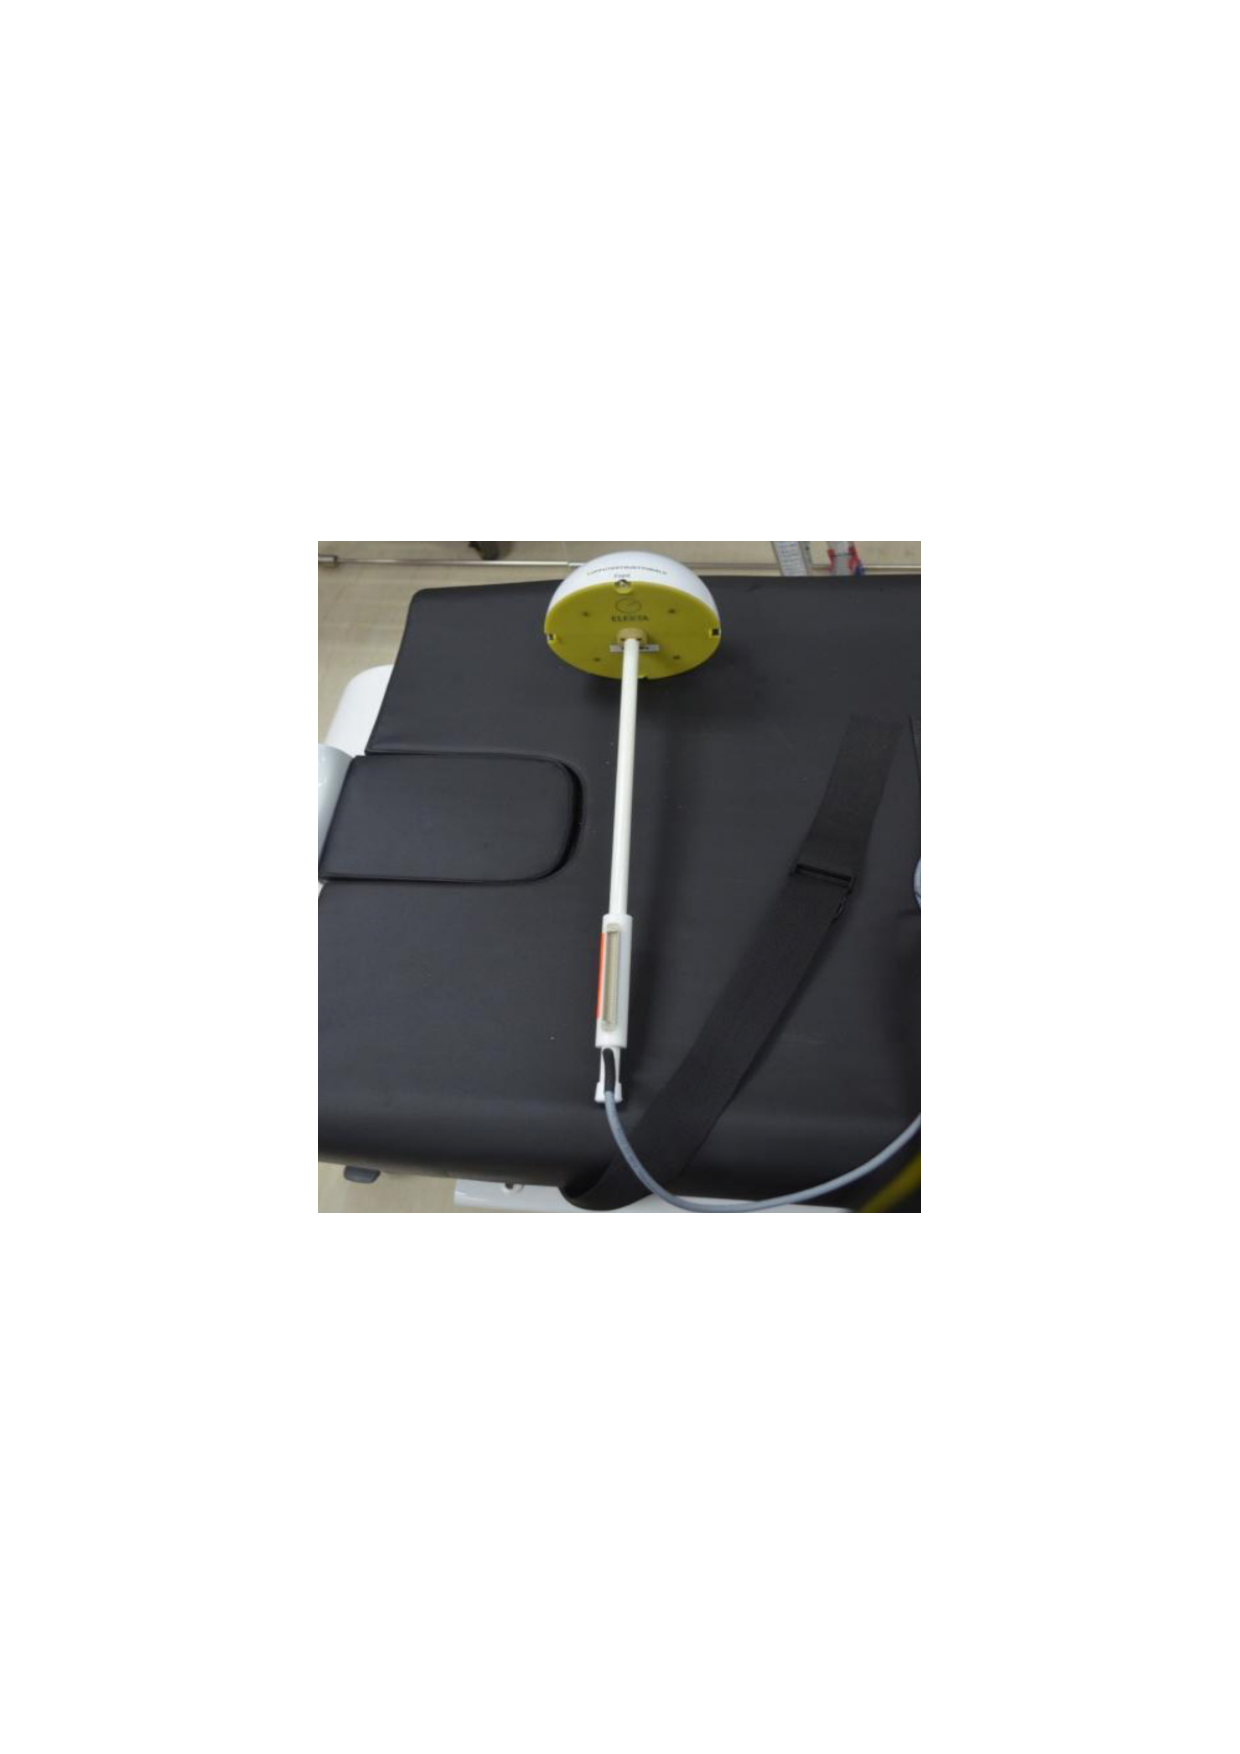
\includegraphics[trim={1cm 8cm 2cm 9cm},width = 0.97\textwidth]{benchmark/phantom_head}
\caption{Reference phantom (RefPhantom) NM24058N (Serial number: 101861) provided by Elekta Oy, Helsinki Finland. 32 built in simulated dipoles and four presetting head position indicator coils (HPI) (Figure taken from~\cite{hazim2015magnetoencephalography}).~\ref{alg:acceptreject}.}
   \label{fig:phantom_head}
\end{figure}

The phantom dipoles are energized using an internal signal generator which also feeds the HPI coils. An external multiplexer box is used to connect the signal to the individual dipoles. Only one dipole can be activated at a time. The location of the dipole is recorded relative to the center of the sphere (0,0,0), where X is positive toward the nasion, Y is positive toward the left ear and Z is positive toward the top of the head.\\

The dataset is sorted into 3 different \ac{SNR}:
\begin{itemize}
\item Source with \textbf{2000 nAm}. This corresponds to an unrealistically strong 1000 nAm (2000 nAm peak-to-peak) dipole that gives the highest SNR of the experimental source.
\item Source with \textbf{200 nAm}. This is a weaker dipole, closer to the range of amplitudes we can expect in raw data.
\item Source with \textbf{20 nAm}. This represents some of the weakest sources we expect in evoked studies which require averaging to detect and estimate (\textit{i.e.} generally cannot be seen in single trial analysis).
\end{itemize}

\subsection{Brainstorm CTF-phantom dataset}

The dataset is sorted into two different SNR:
\begin{itemize}
\item Source with \textbf{200 nAm}. This is a close dipole to the range of amplitudes we can expect in raw data.
\item Source with \textbf{20 nAm}. This represents some of the weakest sources we expect in evoked studies which require averaging to detect and estimate sources (\textit{i.e.} generally cannot be seen in single trial analysis).
\end{itemize}


\begin{figure}[tb]
   \centering
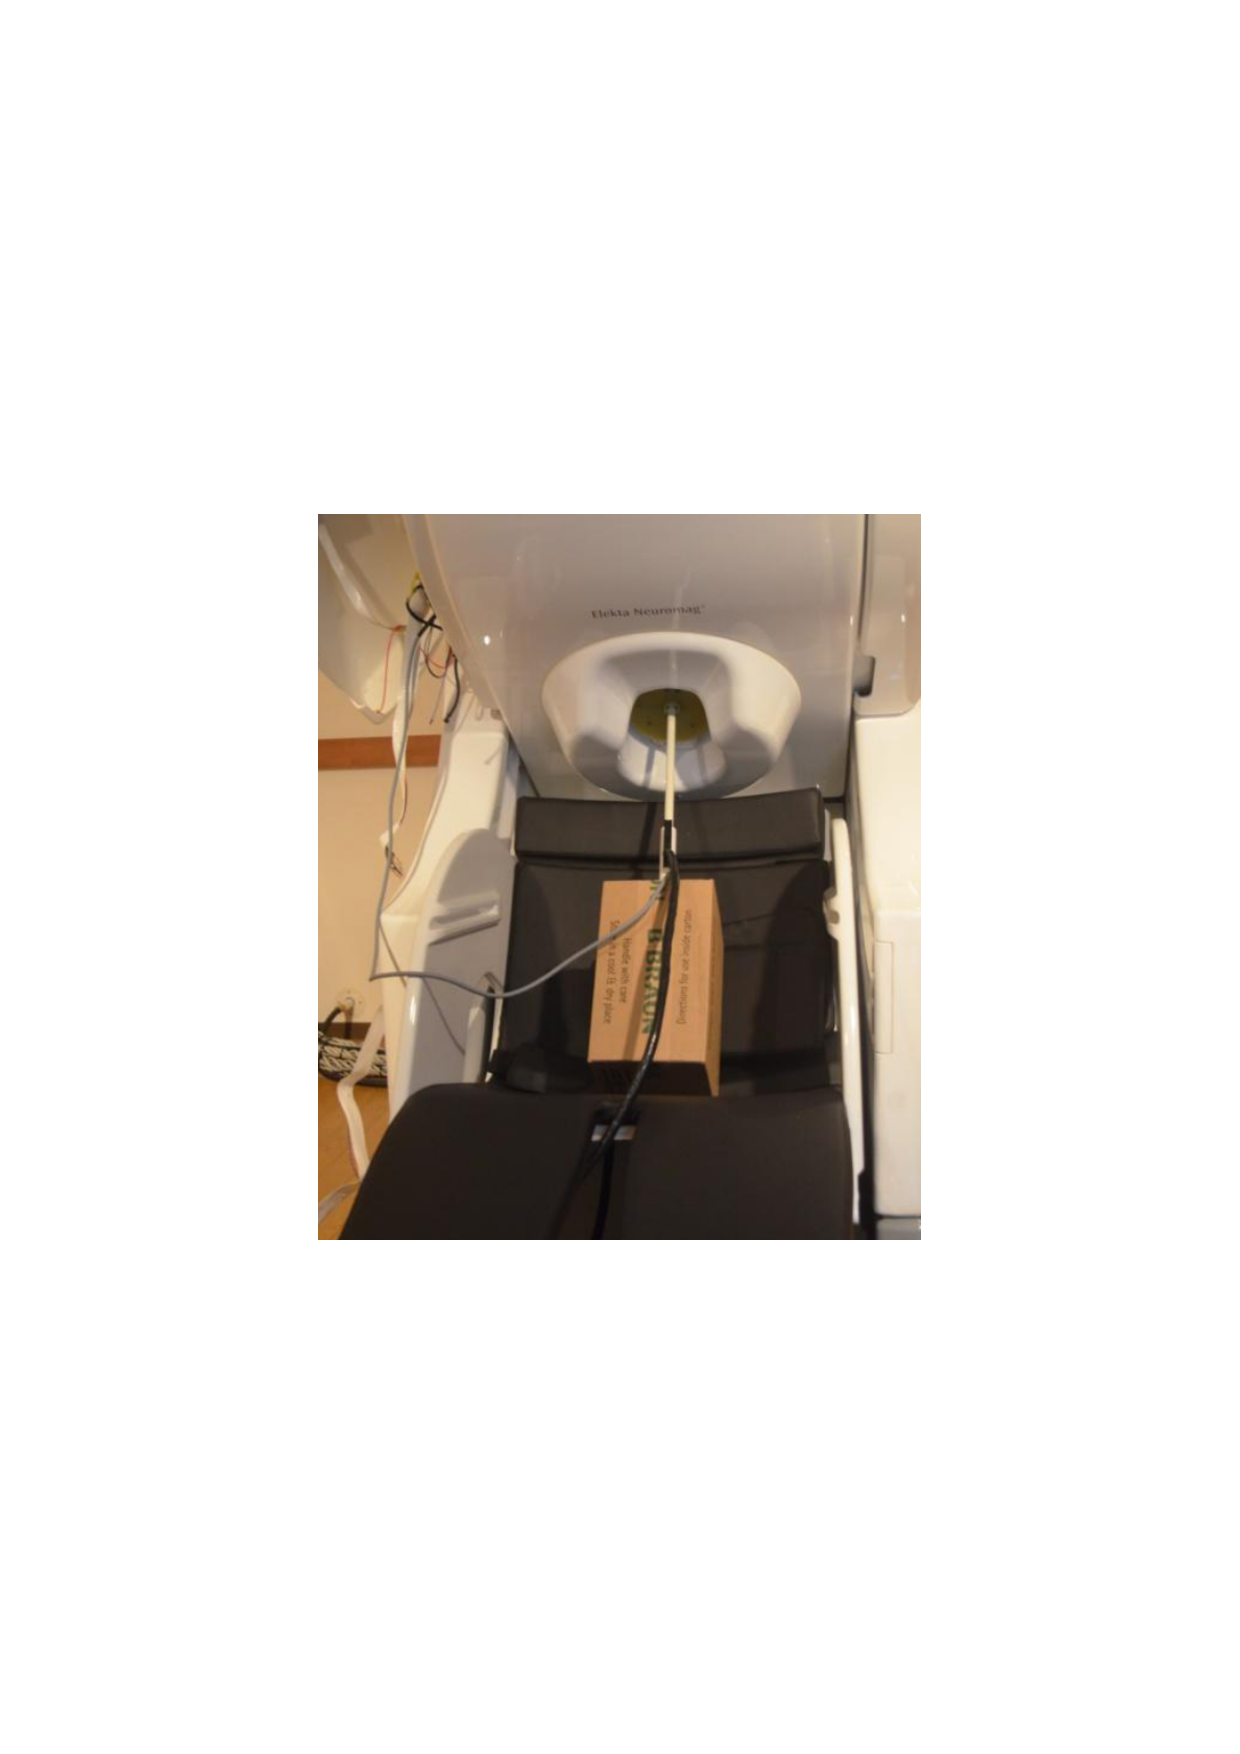
\includegraphics[trim={1cm 8cm 2cm 9cm},width = 0.97\textwidth]{benchmark/phantom_in_MEG}
\caption{Phantom is carefully set into sensor helmet of the probe unit and pushed again helmet. HPI coil is fitted into outlet under right gantry side cover (Figure taken from~\cite{hazim2015magnetoencephalography})~\ref{alg:acceptreject}.}
   \label{fig:phantom_in_MEG}
\end{figure}


\subsection{MNE-Neuromag dataset} \label{data:used_data}

The dataset is sorted into four different SNR:
\begin{itemize}
\item Source with \textbf{2000 nAm}. This corresponds to an unrealistically strong 1000 nAm (2000 nAm peak-to-peak) dipole that gives the highest SNR of the experimental source.
\item Source with \textbf{200 nAm}. This is a weaker dipole, closer to the range of amplitudes we can expect in raw data.
\item Source with \textbf{100 nAm}. This is an even weaker dipole and a smaller SNR.
\item Source with \textbf{20 nAm}. This represents some of the weakest sources we expect in evoked studies which require averaging to detect and estimate sources (\textit{i.e.} generally cannot be seen in single trial analysis).
\end{itemize}

\section{Methodology}

\subsection{Sphere models}
The most commonly used head model assumes that it is made up of a set of nested concentric spheres, each with homogeneous and isotropic conductivity. Under this assumption, both the EEG and MEG problems have well known closed form solutions~\cite{mosher1999eeg}.

\subsection{The selected solvers}
\subsubsection{Dipole fitting}
Dipole fitting assumes that a small number of point-like \ac{ECD}s can describe the measured topography. It optimises the location, the orientation and the amplitude of the model dipoles in order to minimise the difference between the model and the measured topography. A good introduction to dipole fitting is provided by~\cite{scherg1990fundamentals}. A full description is done in Chapter~\ref{chapter:background}-Section~\ref{section_dipfit}.

\subsubsection{$\gamma$-Map}
$\gamma$-map offers a unifying view using a Bayesian perspective on some of the solvers presented here. As it was shown in Chapter~\ref{chapter:bayesian}, the Bayesian formulation of the MEG/EEG source localization consists in choosing priors/hyperpriors, estimation and inference procedure where often it boils down to alternating between the estimation of the source estimate and the estimation of the hyperparameter. The hyperparameter in this method is $\gamma$ which represents covariance components. More details are in~\cite{Wipf-Nagarajan:2009}.

\subsubsection{RAP-MUSIC}
\Ac{RAP-MUSIC} is an extension to \ac{MUSIC} by recursively estimating multiple sources~\cite{mosher1997source,mosher1999source}. In other words, it consists in applying MUSIC successively after removing the contribution of the previously identified sources. Such as matching pursuit algorithms are used for sparse signal decomposition over dictionary of atoms, the RAP-MUSIC method adopts a greedy strategy to select the relevant dipoles in a dictionary of sources.

\subsubsection{MxNE | irMxNE}
\Ac{MxNE} and \ac{irMxNE} are the convex and the non-convex version of mixed-norms solvers using $\ell_{2,1}$-norm and $\ell_{2,0.5}$-quasinorm as regularizations. For more details, see Chapter~\ref{chapter:background}-Section~\ref{sec:mixed_norms} and~\cite{gramfort2012mixed,strohmeier-etal:16}.

\subsubsection{TF-MxNE | irTF-MxNE}
\Ac{TF-MxNE} and \ac{irTF-MxNE} are the convex and the non-convex version of the Time-Frequency mixed-norms using $\ell_{2,1}+\ell_1$-norm and $\ell_{2,0.5}+\ell_{0.5}$-quasinorm as regularizations. For more details, see  see Chapter~\ref{chapter:background}-Section~\ref{sec:mixed_norms} and~\cite{TF-MxNE,bekhti2016m}.

\section{Experimental results}
Three types of errors have been investigated for the different solvers, namely: the position or location error, orientation error, and amplitude error. All the solvers investigated here are implemented in the MNE-python package~\cite{mne-python,mne}.

The position error $err_{pos}$ is represented in millimeters (mm), defining the distance between the exact location ($pos_{simulated}\in\RR^3$) of the simulated dipole in the phantom head and the estimated location ($pos_{estimated}\in\RR^3$) as in Equation~\eqref{eq:pos_err}. When the estimated source space contains multiple dipoles, the one having the biggest peak of amplitude is kept and compared to the exact dipole.

\begin{equation}\label{eq:pos_err}
err_{pos} = 10^3 \|pos_{estimated} - pos{simulated}\|_{Fro}
\end{equation}

The orientation error $err_{ori}$ is represented in Radians (Rad), defining the angle between the exact orientation ($ori_{simulated}\in\RR^3$) of the simulated dipole and the estimated one ($ori_{estimated}\in\RR^3$) as in Equation~\eqref{eq:ori_err}. Same for the position error, the best dipole is kept when multiple ones are estimated.

\begin{equation}\label{eq:ori_err}
err_{ori} = arccos(|<ori_{estimated}, ori_{simulated}>|)
\end{equation}

Finally, the amplitude error $err_{amp}$is represented in nanoAmpere (nAm) except for some solvers which give source estimates with statistical values and not electrical current values (example: dSPM). This error defines the difference between the peak of amplitude ($max(amp_{estimated}) with amp_{estimated}\in\RR^T$) of the estimated dipole and the peak of simulated dipole $amp_{simulated}\in\RR$ (example 1000nAm, 200nAm, ... 20nAm) as in Equation~\eqref{eq:amp_err}.

\begin{equation}\label{eq:amp_err}
err_{amp} = |max(amp_{estimated} - amp_{simulated})|
\end{equation}

Figures showing the three types of error over different solvers are displayed below. On the x-axis, three different pre-processing types are presented:
\begin{itemize}
\item \textit{Raw}: the source localization is using the raw data without applying maxfilter.
\item \textit{SSS}: the source localization is applying Signal Space Separation (SSS), also known as maxfilter. It is the first step of preprocessing MEG data, which is a clever mathematical way to separate magnetic signals coming from the brain from those coming from outside the brain.
\item \textit{$SSS_{MNE}$}: the source localization is applying a new implementation of maxfilter in MNE-python.
\end{itemize}

Figure~\ref{fig:dipfit_errors} shows position errors obtained with dipole fitting method for the 4 simulated dipoles (dataset \ref{data:used_data}) and for the different SNRs. Figure~\ref{fig:dipfit_pos} shows less than 1mm error for the unrealistic high SNR (peak-to-peak amplitude equal to 1000nAm), but also for 200nAM, and 100nAm. The location error gets worse with the very low SNR (20nAm).
%\subsection*{dipfit}

\begin{sidewaysfigure}[ht]
        \centering
        \begin{subfigure}[b]{0.28\textwidth}
            \centering
            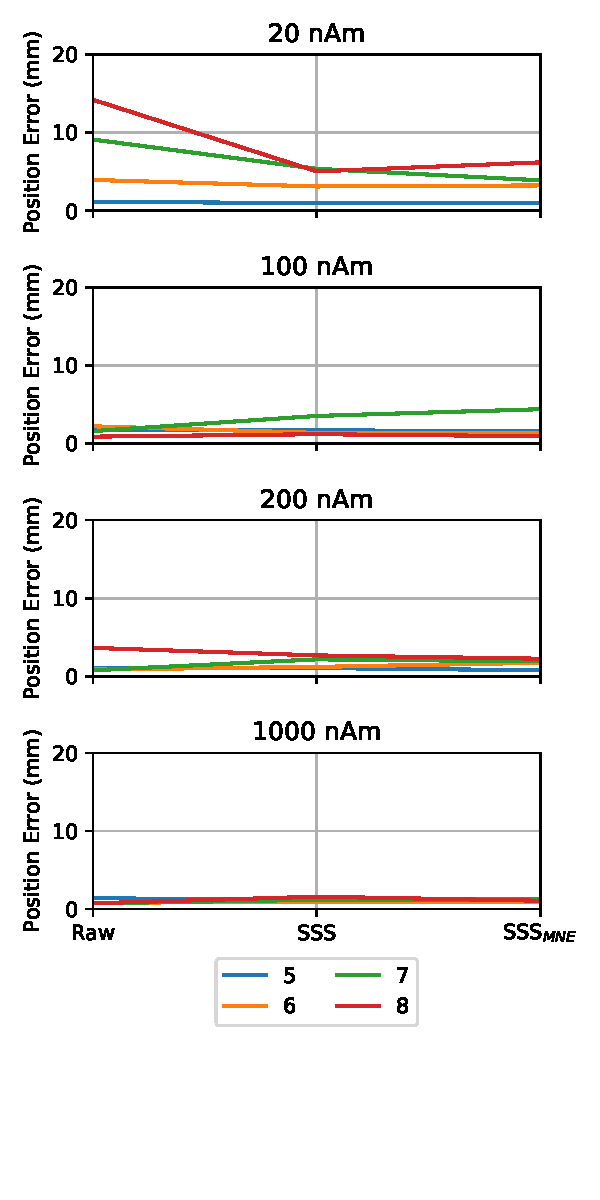
\includegraphics[trim={1cm 2.5cm 1cm 1cm},width=\textwidth]{benchmark/phantom_errors_dipfit_loc_error}
            \caption{\label{fig:dipfit_pos}}
        \end{subfigure}
		\hspace{35pt}
        \begin{subfigure}[b]{0.28\textwidth}  
            \centering 
            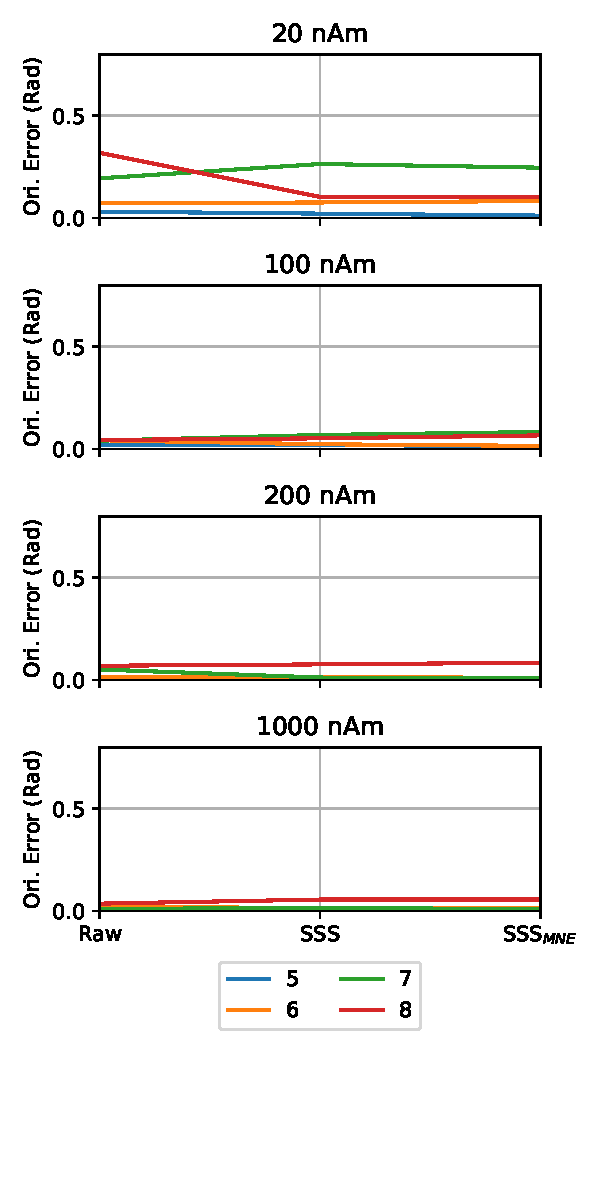
\includegraphics[trim={1cm 2.5cm 1cm 1cm},width=\textwidth]{benchmark/phantom_errors_dipfit_ori_error}
            \caption{\label{fig:dipfit_ori}}
        \end{subfigure}
		\hspace{35pt}
        \begin{subfigure}[b]{0.28\textwidth}   
            \centering 
            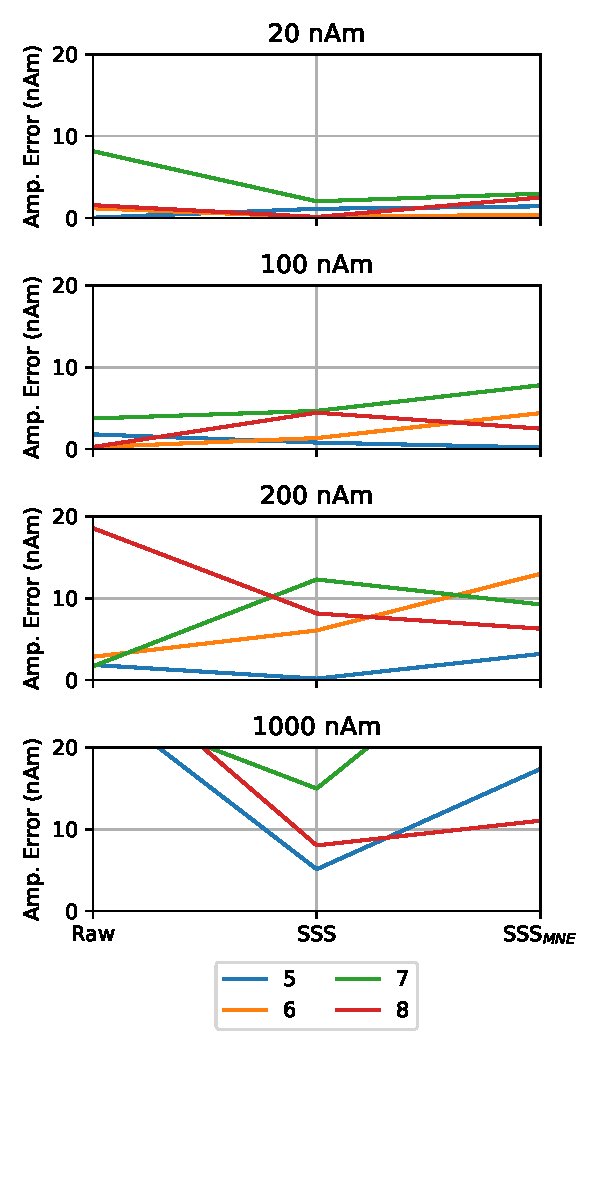
\includegraphics[trim={1cm 2.5cm 1cm 1cm},width=\textwidth]{benchmark/phantom_errors_dipfit_amp_error}
            \caption{\label{fig:dipfit_amp}}
        \end{subfigure}

		\caption{The dipole fit errors on localization (mm), orientation (Rad), and amplitude (nAm) using 4 dipoles (5-8) having different depth in the phantom.\label{fig:dipfit_errors}}
\end{sidewaysfigure}

Dipole fitting approach is very suitable to localize the neuronal activity when a small number of \ac{ECD}s can describe the data. In this dataset \ref{data:used_data}, each dipole is recorded alone. The errors in orientations and amplitude are in Figure \ref{fig:dipfit_ori}-\ref{fig:dipfit_amp}.

RAP-MUSIC is an approach based on MUSIC technique which also perform very well when few ECDs are involved, especially when it is a dataset recording only one dipole in a row. It can be seen as very competitive to dipole fitting in Figure \ref{fig:music_pos}-\ref{fig:music_ori}-\ref{fig:music_amp} showing the errors in position, orientation, and amplitude respectively. However, for deep source (dipole 8) combined with very low SNR (20nAm) the red curve is outside of the box meaning a location error bigger than 20mm. This is an issue with the signal subspace estimation, where the rank of the data covariance is not being well estimated.

%\subsection*{MUSIC}
\begin{sidewaysfigure}[ht]
        \centering
        \begin{subfigure}[b]{0.28\textwidth}
            \centering
            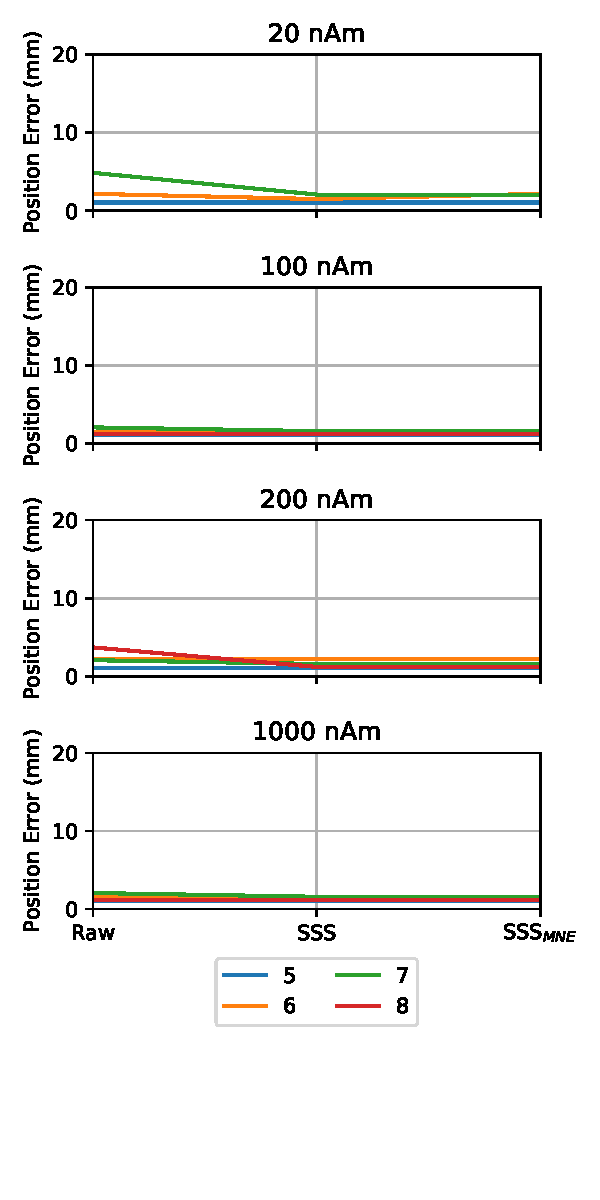
\includegraphics[trim={1cm 2.5cm 1cm 1cm},width=\textwidth]{benchmark/phantom_errors_music_loc_error}
            \caption{\label{fig:music_pos}}
        \end{subfigure}
		\hspace{35pt}
        \begin{subfigure}[b]{0.28\textwidth}  
            \centering 
            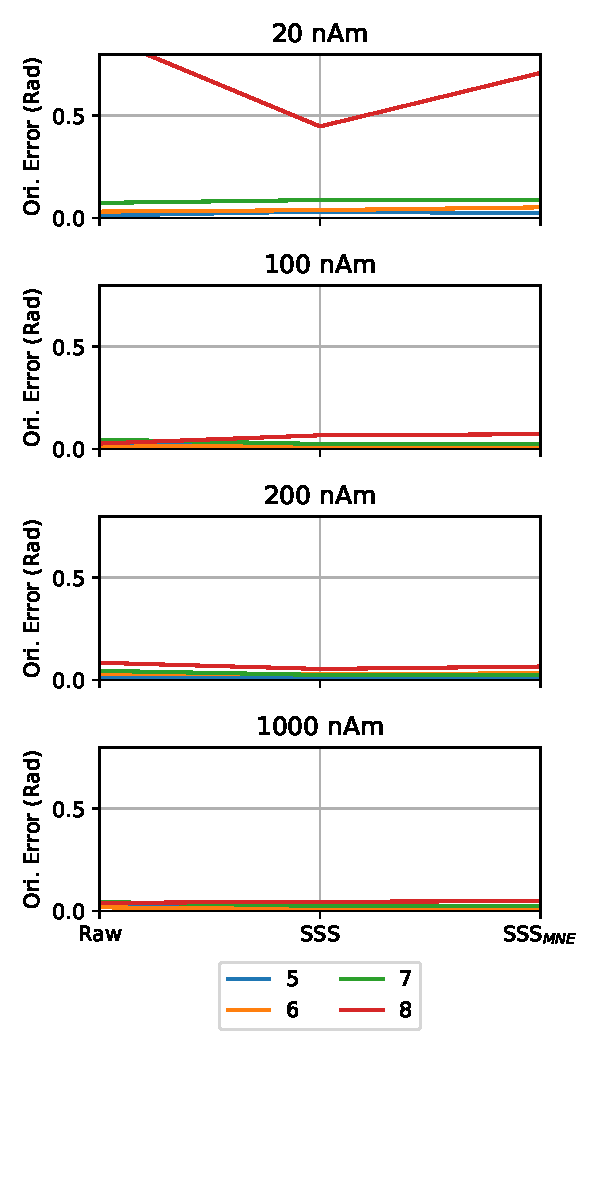
\includegraphics[trim={1cm 2.5cm 1cm 1cm},width=\textwidth]{benchmark/phantom_errors_music_ori_error}
            \caption{\label{fig:music_ori}}
        \end{subfigure}
		\hspace{35pt}
        \begin{subfigure}[b]{0.28\textwidth}   
            \centering 
            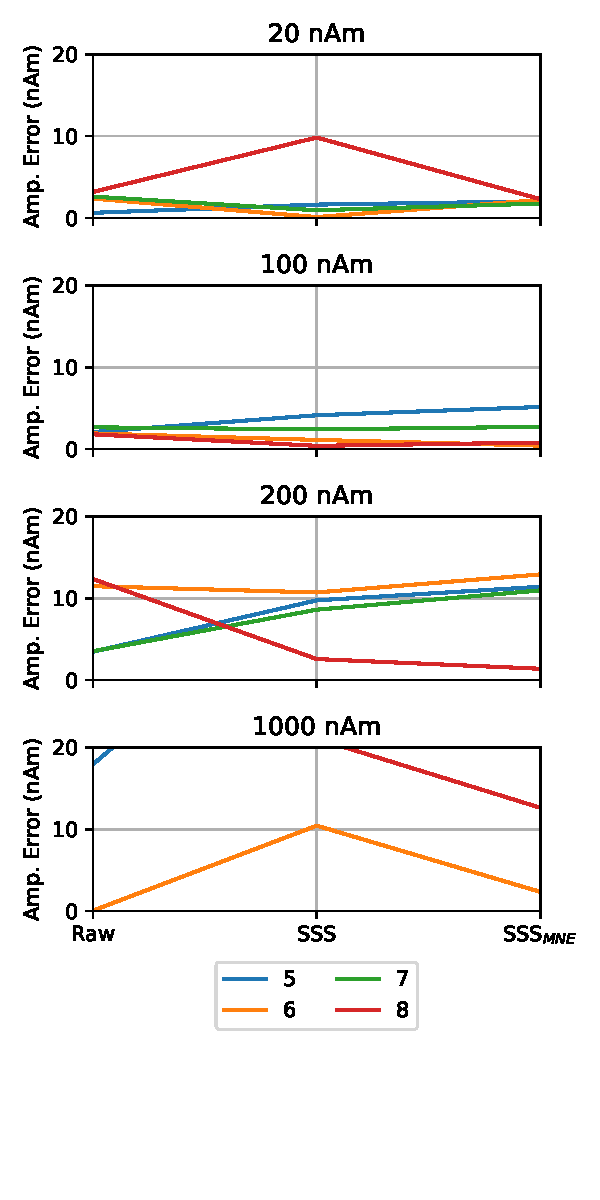
\includegraphics[trim={1cm 2.5cm 1cm 1cm},width=\textwidth]{benchmark/phantom_errors_music_amp_error}
            \caption{\label{fig:music_amp}}
        \end{subfigure}

		\caption{The MUSIC errors on localization (mm), orientation (Rad), and amplitude (nAm) using 4 dipoles (5-8) having different depth in the phantom.\label{fig:music_errors}}
\end{sidewaysfigure}


%\subsection*{Gamma map}
\begin{sidewaysfigure}[ht]
        \centering
%        \vspace{10pt}
        \begin{subfigure}[b]{0.28\textwidth}
            \centering
            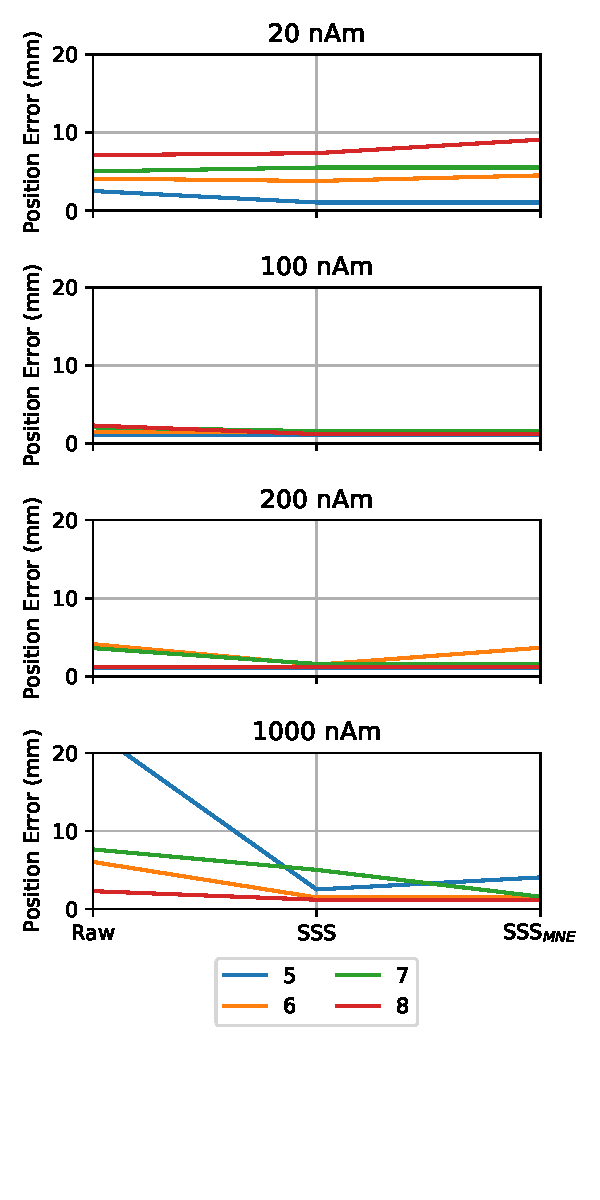
\includegraphics[trim={1cm 2.5cm 1cm 1cm},width=\textwidth]{benchmark/phantom_errors_gamma_map_loc_error}
            \caption{\label{fig:gmap_pos}}
        \end{subfigure}
%        \hfill
		\hspace{35pt}
        \begin{subfigure}[b]{0.28\textwidth}  
            \centering 
            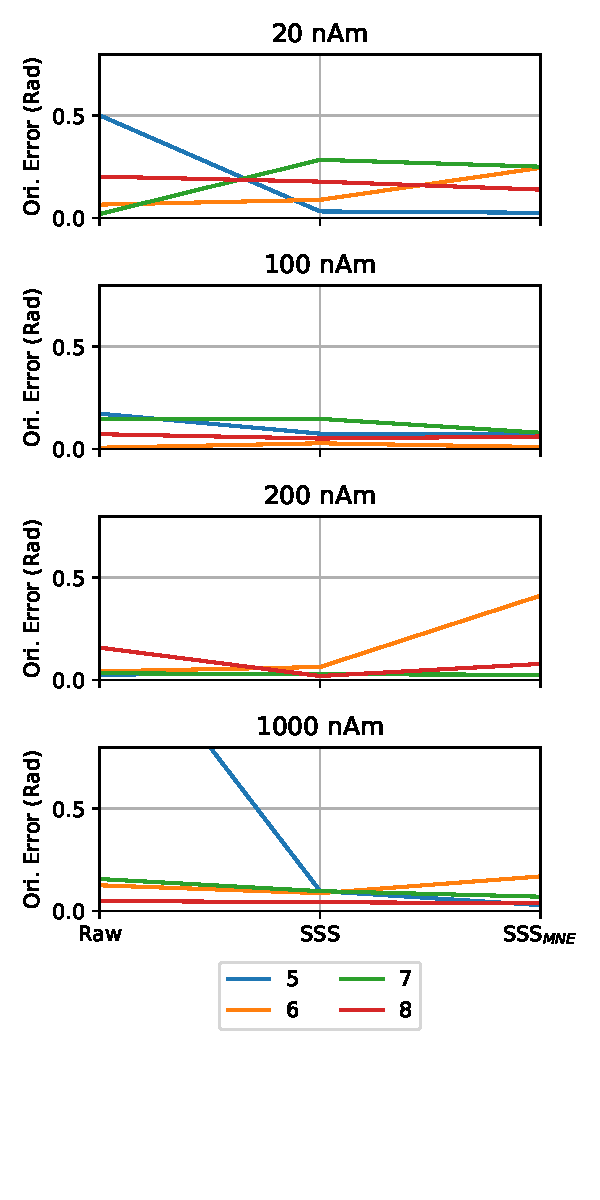
\includegraphics[trim={1cm 2.5cm 1cm 1cm},width=\textwidth]{benchmark/phantom_errors_gamma_map_ori_error}
            \caption{\label{fig:gmap_ori}}
        \end{subfigure}
%        \vskip\baselineskip
		\hspace{35pt}
        \begin{subfigure}[b]{0.28\textwidth}   
            \centering 
            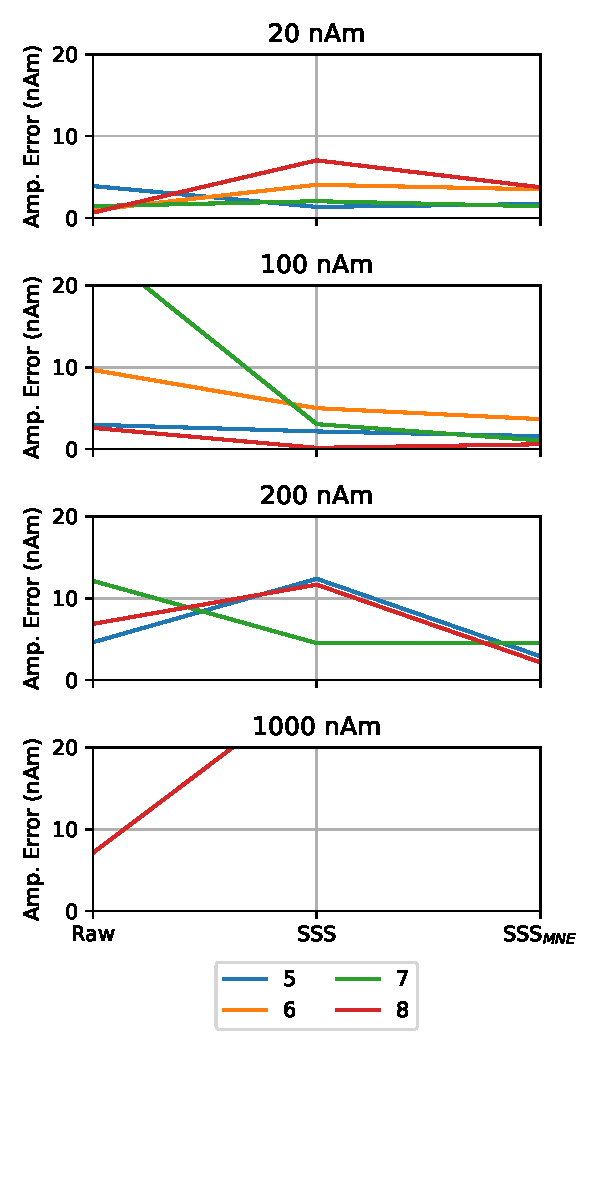
\includegraphics[trim={1cm 2.5cm 1cm 1cm},width=\textwidth]{benchmark/phantom_errors_gamma_map_amp_error}
            \caption{\label{fig:gmap_amp}}
        \end{subfigure}

		\caption{The gamma map errors on localization (mm), orientation (Rad), and amplitude (nAm) using 4 dipoles (5-8) having different depth in the phantom.\label{fig:gmap_errors}}
\end{sidewaysfigure}


%\subsection*{Mixed norm (MxNE)}
\begin{sidewaysfigure}[ht]
        \centering
%        \vspace{10pt}
        \begin{subfigure}[b]{0.28\textwidth}
            \centering
            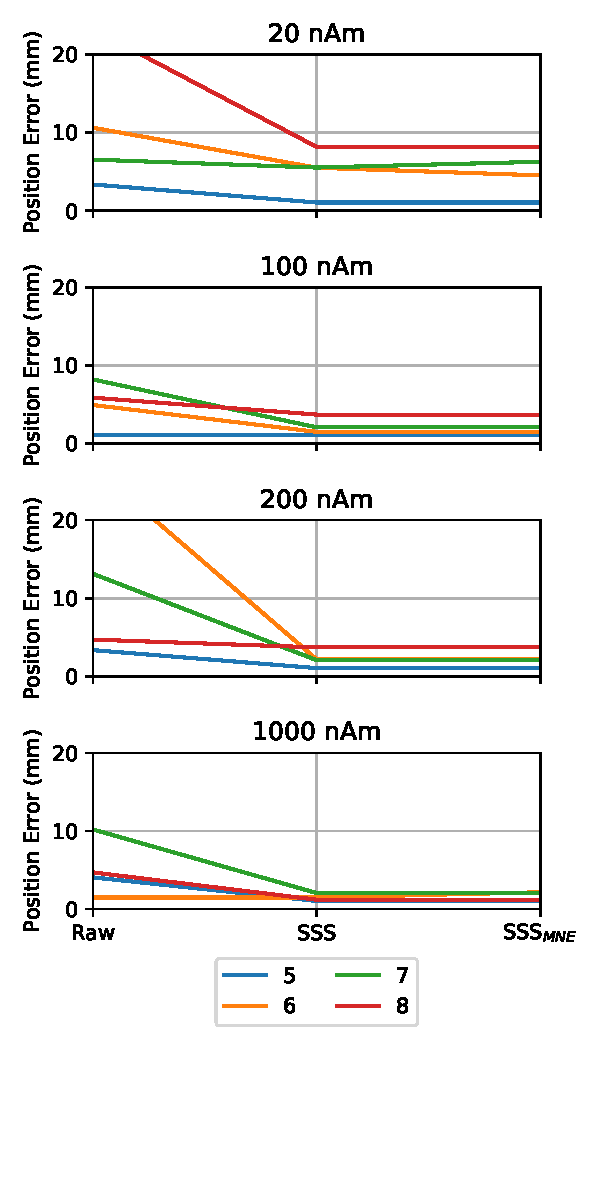
\includegraphics[trim={1cm 2.5cm 1cm 1cm},width=\textwidth]{benchmark/phantom_errors_MxNE_loc_error}
            \caption{\label{fig:mxne_pos}}
        \end{subfigure}
		\hspace{35pt}
        \begin{subfigure}[b]{0.28\textwidth}  
            \centering 
            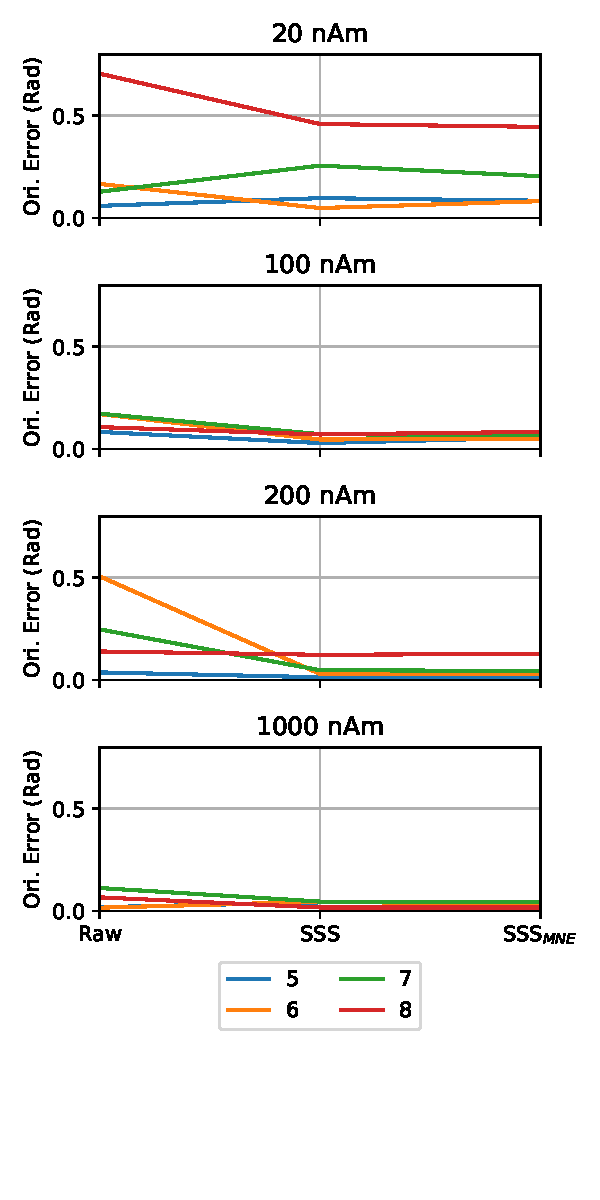
\includegraphics[trim={1cm 2.5cm 1cm 1cm},width=\textwidth]{benchmark/phantom_errors_MxNE_ori_error}
            \caption{\label{fig:mxne_ori}}
        \end{subfigure}
		\hspace{35pt}
        \begin{subfigure}[b]{0.28\textwidth}   
            \centering 
            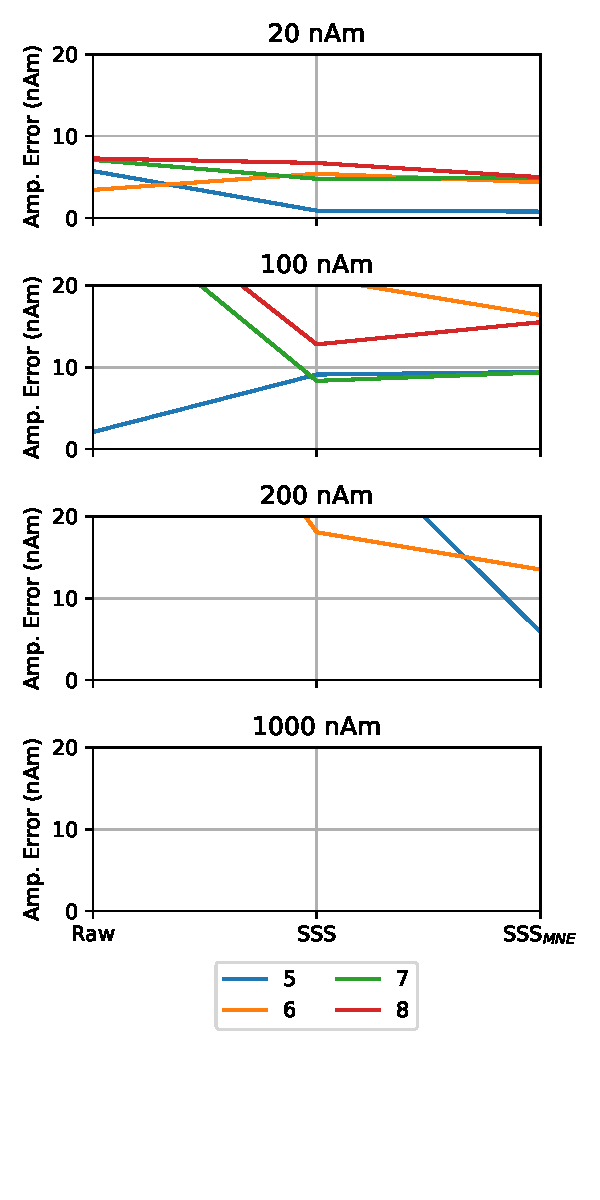
\includegraphics[trim={1cm 2.5cm 1cm 1cm},width=\textwidth]{benchmark/phantom_errors_MxNE_amp_error}
            \caption{\label{fig:mxne_amp}}
        \end{subfigure}

		\caption{The mixed norm (MxNE) errors on localization (mm), orientation (Rad), and amplitude (nAm) using 4 dipoles (5-8) having different depth in the phantom.\label{fig:gmap_errors}}
\end{sidewaysfigure}

%\subsection*{Time-Frequency mixed-norm (TF-MxNE)}
\begin{sidewaysfigure}[ht]
        \centering
        \begin{subfigure}[b]{0.28\textwidth}
            \centering
            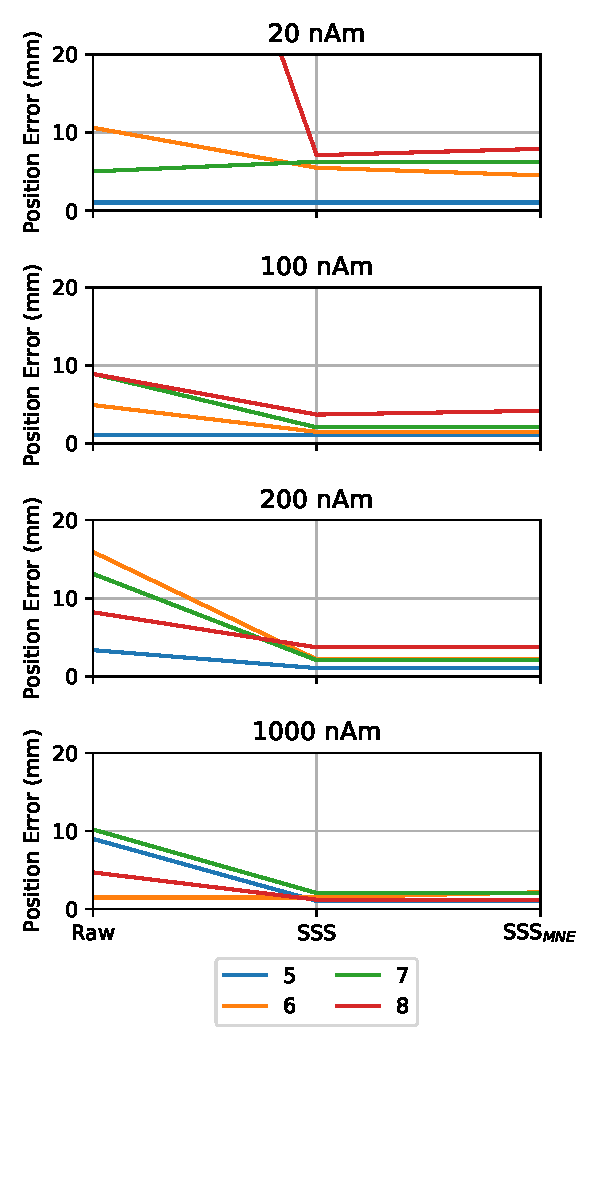
\includegraphics[trim={1cm 2.5cm 1cm 1cm},width=\textwidth]{benchmark/phantom_errors_TF-MxNE_depth_95_wsize_64_tstep_16_40_1_loc_error}
            \caption{\label{fig:tfmxne_pos}}
        \end{subfigure}
		\hspace{35pt}
        \begin{subfigure}[b]{0.28\textwidth}  
            \centering 
            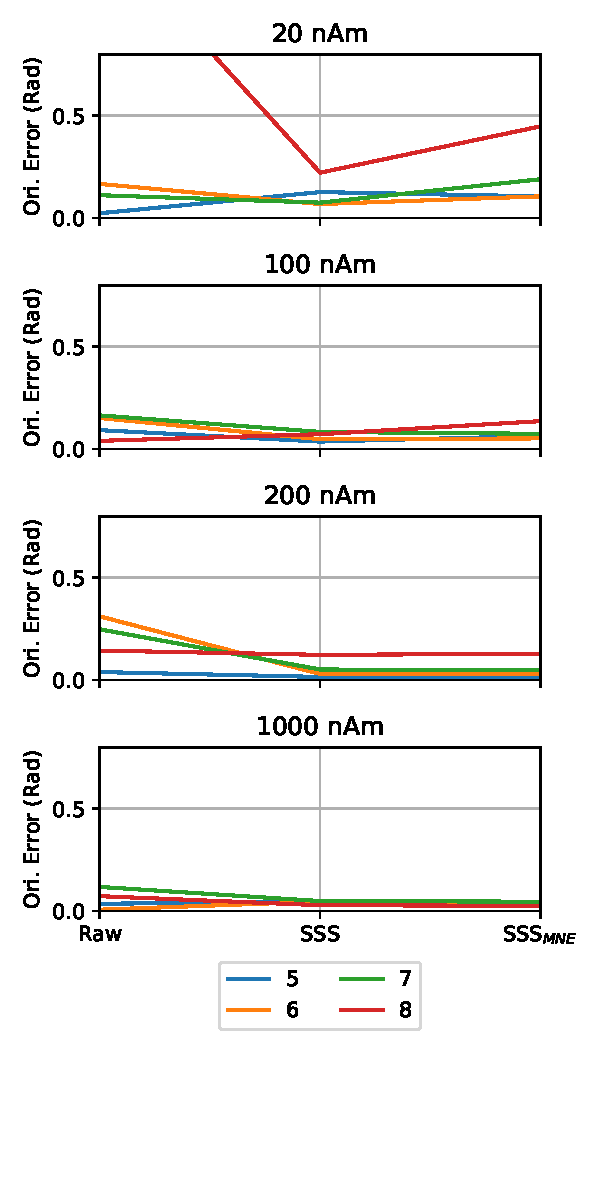
\includegraphics[trim={1cm 2.5cm 1cm 1cm},width=\textwidth]{benchmark/phantom_errors_TF-MxNE_depth_95_wsize_64_tstep_16_40_1_ori_error}
            \caption{\label{fig:tfmxne_ori}}
        \end{subfigure}
		\hspace{35pt}
        \begin{subfigure}[b]{0.28\textwidth}   
            \centering 
            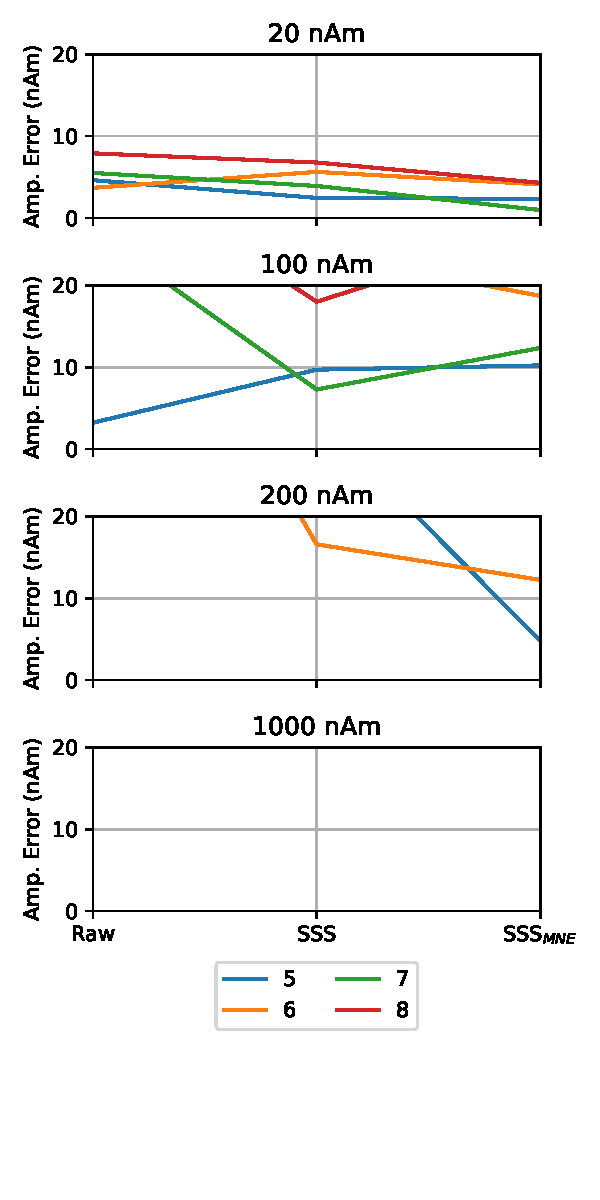
\includegraphics[trim={1cm 2.5cm 1cm 1cm},width=\textwidth]{benchmark/phantom_errors_TF-MxNE_depth_95_wsize_64_tstep_16_40_1_amp_error}
            \caption{\label{fig:tfmxne_amp}}
        \end{subfigure}

		\caption{The time-frequency mixed-norm (TF-MxNE) errors on localization (mm), orientation (Rad), and amplitude (nAm) using 4 dipoles (5-8) having different depth in the phantom.\label{fig:tfmxne_errors}}
\end{sidewaysfigure}

$\gamma$-map which is a Bayesian formulation to the MEG/EEG inverse problem is performing less well than dipole fitting or RAP-MUSIC for very high and very low SNR. For SNRs in range of realistic data, its location error is majored by 5mm depending on the depth of the studied dipole. $\gamma$-map is doing worse for amplitude=1000nAm compared to 100nAm or 200nAm because it overestimates the noise when estimating the hyperparameter $\gamma$.

For MxNE and TF-MxNE, the errors shown in Figure~\ref{fig:mxne_pos}-\ref{fig:tfmxne_pos} respectively demonstrate an improvement when using TF-MxNE.

\subsection{Critical comparison of these MEG/EEG source localization}
Figure \ref{all_solvers_loc_error} shows all solvers in the same plot to compare both errors in location and orientation with maxfilter as preprocessing. We keep the same scale for y-axis to not go beyond 20 mm of location error and not beyond 1 Rad of orientation error. The left plot of location error shows firstly (RAP) MUSIC as being very sensitive the SNR (comparing 20nAm to 1000nAm). Then MNE and dSPM as the methods giving the worst results for this dataset. One important argument is the fact that the study is biased as we know that the simulated phantom data is focal/sparse, while MNE and dSPM are not sparse methods. We always take the peak of amplitude and displays the best dipole for each method. sLORETA in the other hand is not a sparse method either, however, it performs much better than MNE or dSPM. The "center" of the pattern estimated with sLORETA is then closer to the exact dipole location compared to the center of dSPM or MNE. TF-MxNE is not the best method for this study as it is a spatio-temporal approach when having a specific waveforms in the data which is not the case here.

\begin{sidewaysfigure}[ht]
        \centering
        \begin{subfigure}[b]{0.47\textwidth}
            \centering
            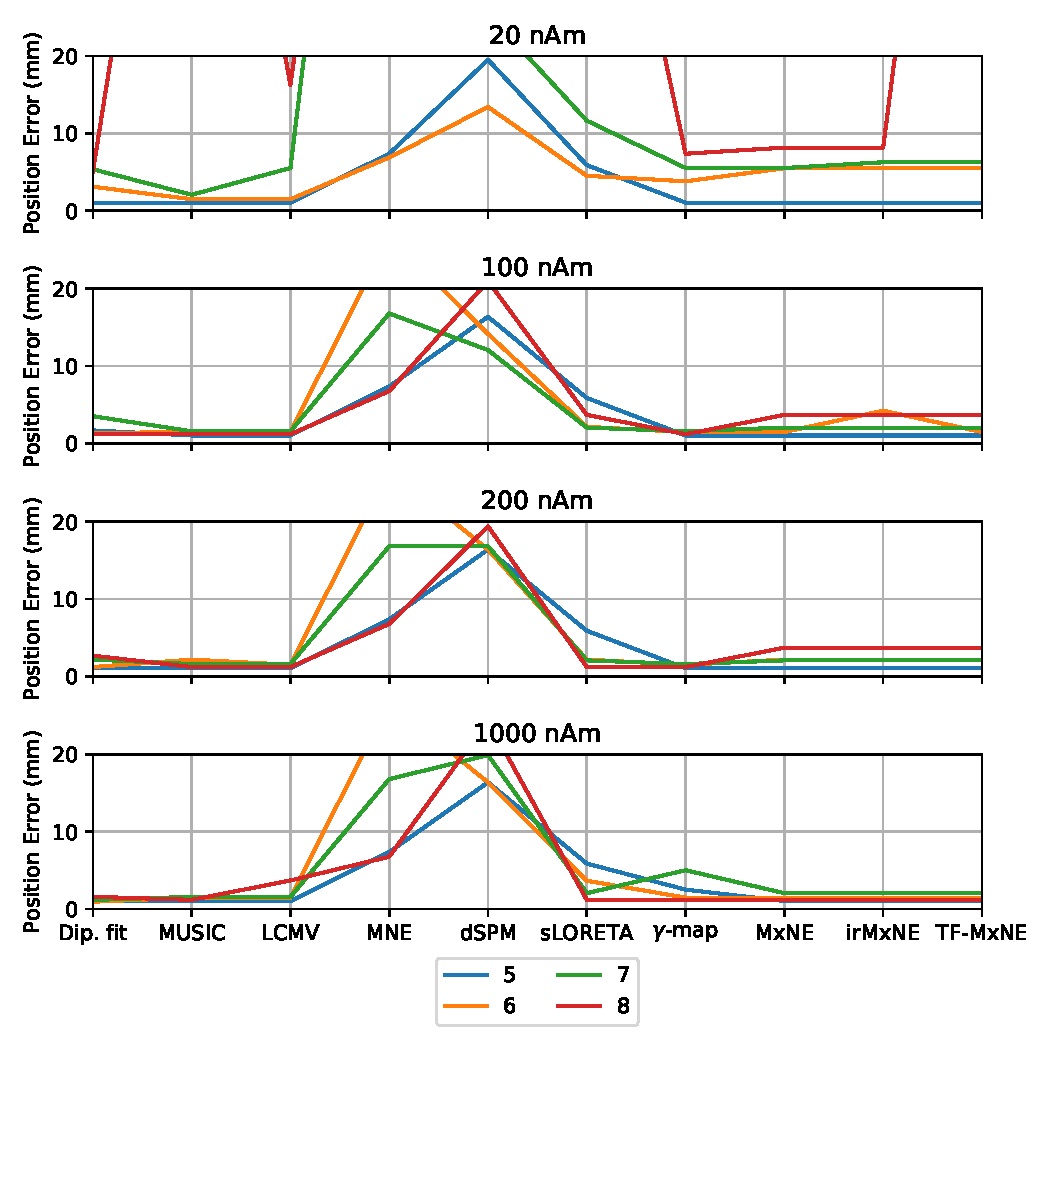
\includegraphics[trim={1cm 2.5cm 1cm 1cm},width=\textwidth]{benchmark/phantom_errors_all_solvers_maxfilter_True_loc_error}
            \caption{\label{fig:all_solvers_loc_error}}
        \end{subfigure}
		\hspace{25pt}
        \begin{subfigure}[b]{0.47\textwidth}  
            \centering 
            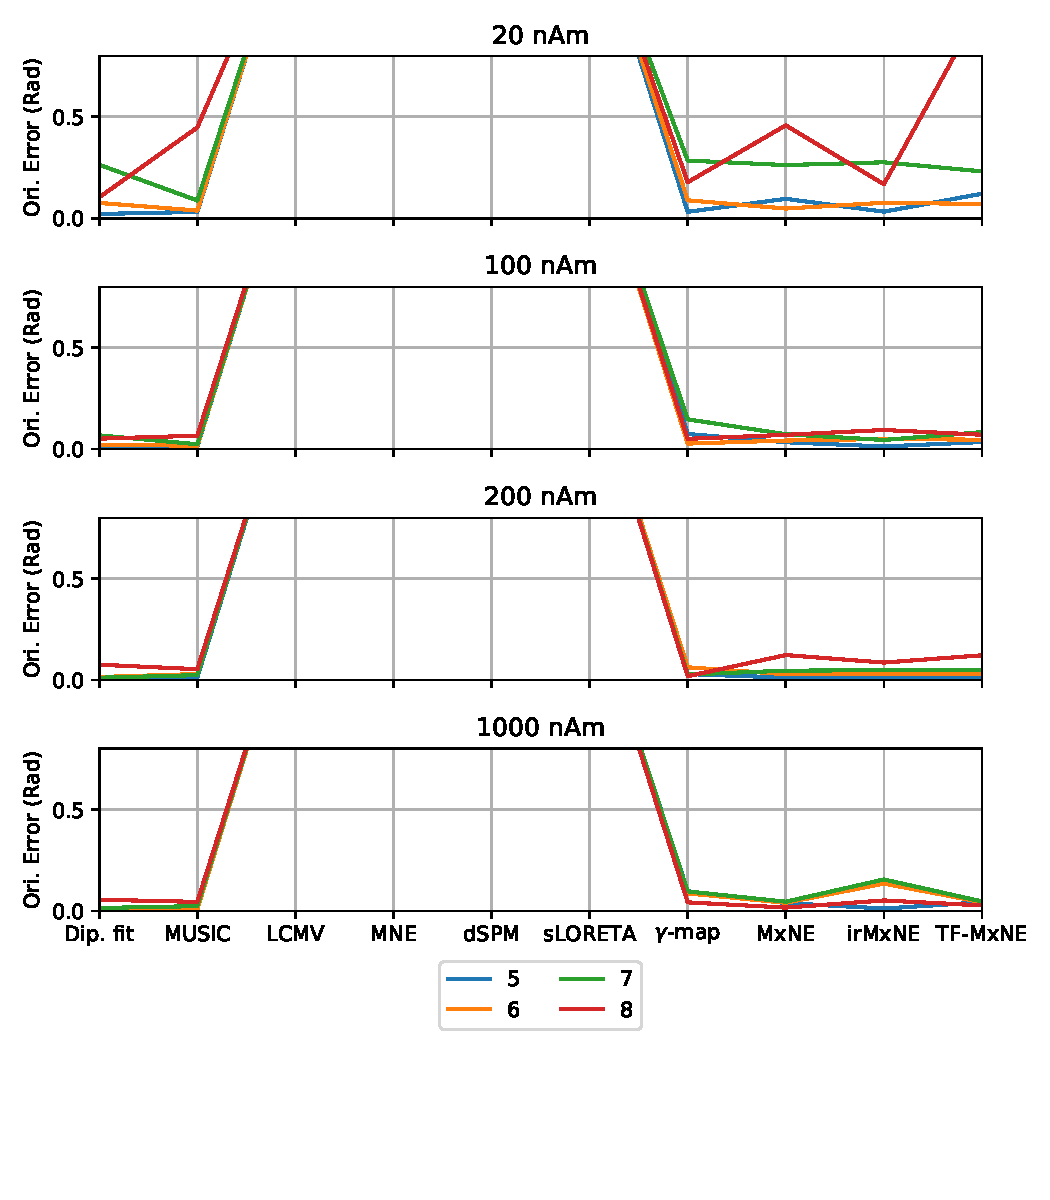
\includegraphics[trim={1cm 2.5cm 1cm 1cm},width=\textwidth]{benchmark/phantom_errors_all_solvers_maxfilter_True_ori_error}
            \caption{\label{fig:all_solvers_ori_error}}
        \end{subfigure}

		\caption{Comparison of the position and the orientation error between most of the solvers for 4 different dipoles.\label{all_solvers_loc_error}}
\end{sidewaysfigure}

The orientation error is comparable to the location error, where dipole fitting, MUSIC, $\gamma$-map, MxNE and irMxNE keeps being the best performing methods. Dipole fitting is unbeatable when simulating with only one dipole. We could not sum up dipoles to make the simulation even harder, because their locations is nearly the same except the depth is different. When summing up this type of dipole, they still have the same pattern in the sensor space, which makes the source localization impossible.

\begin{figure}
	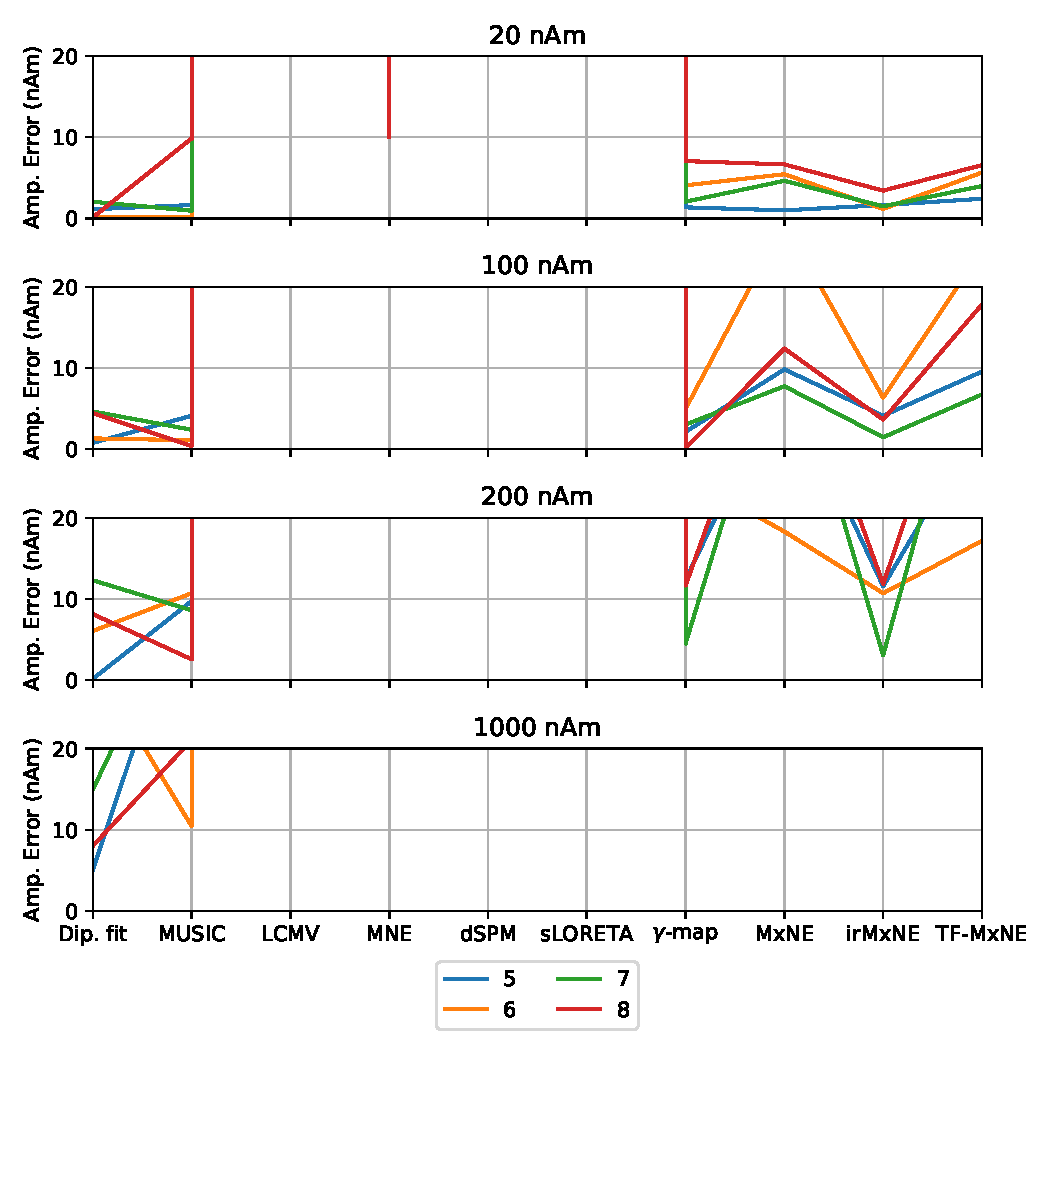
\includegraphics[width=\textwidth]{benchmark/phantom_errors_all_solvers_maxfilter_True_amp_error}
	\caption{Comparison of amplitude error between most of the solvers for 4 different dipoles.\label{all_solvers_amp_error}}
\end{figure}

Figure~\ref{all_solvers_amp_error} shows the errors in amplitude, the most important point in this figure is to see the difference between the convex MxNE and the non-convex irMxNE in terms of amplitude bias. All dipoles basically improve their amplitude estimate when using the non-convex method (irMxNE). For some cases, irMxNE amplitude estimate is even better than dipole fitting one.

\begin{sidewaysfigure}[ht]
        \centering
        \begin{subfigure}[b]{0.47\textwidth}
            \centering
            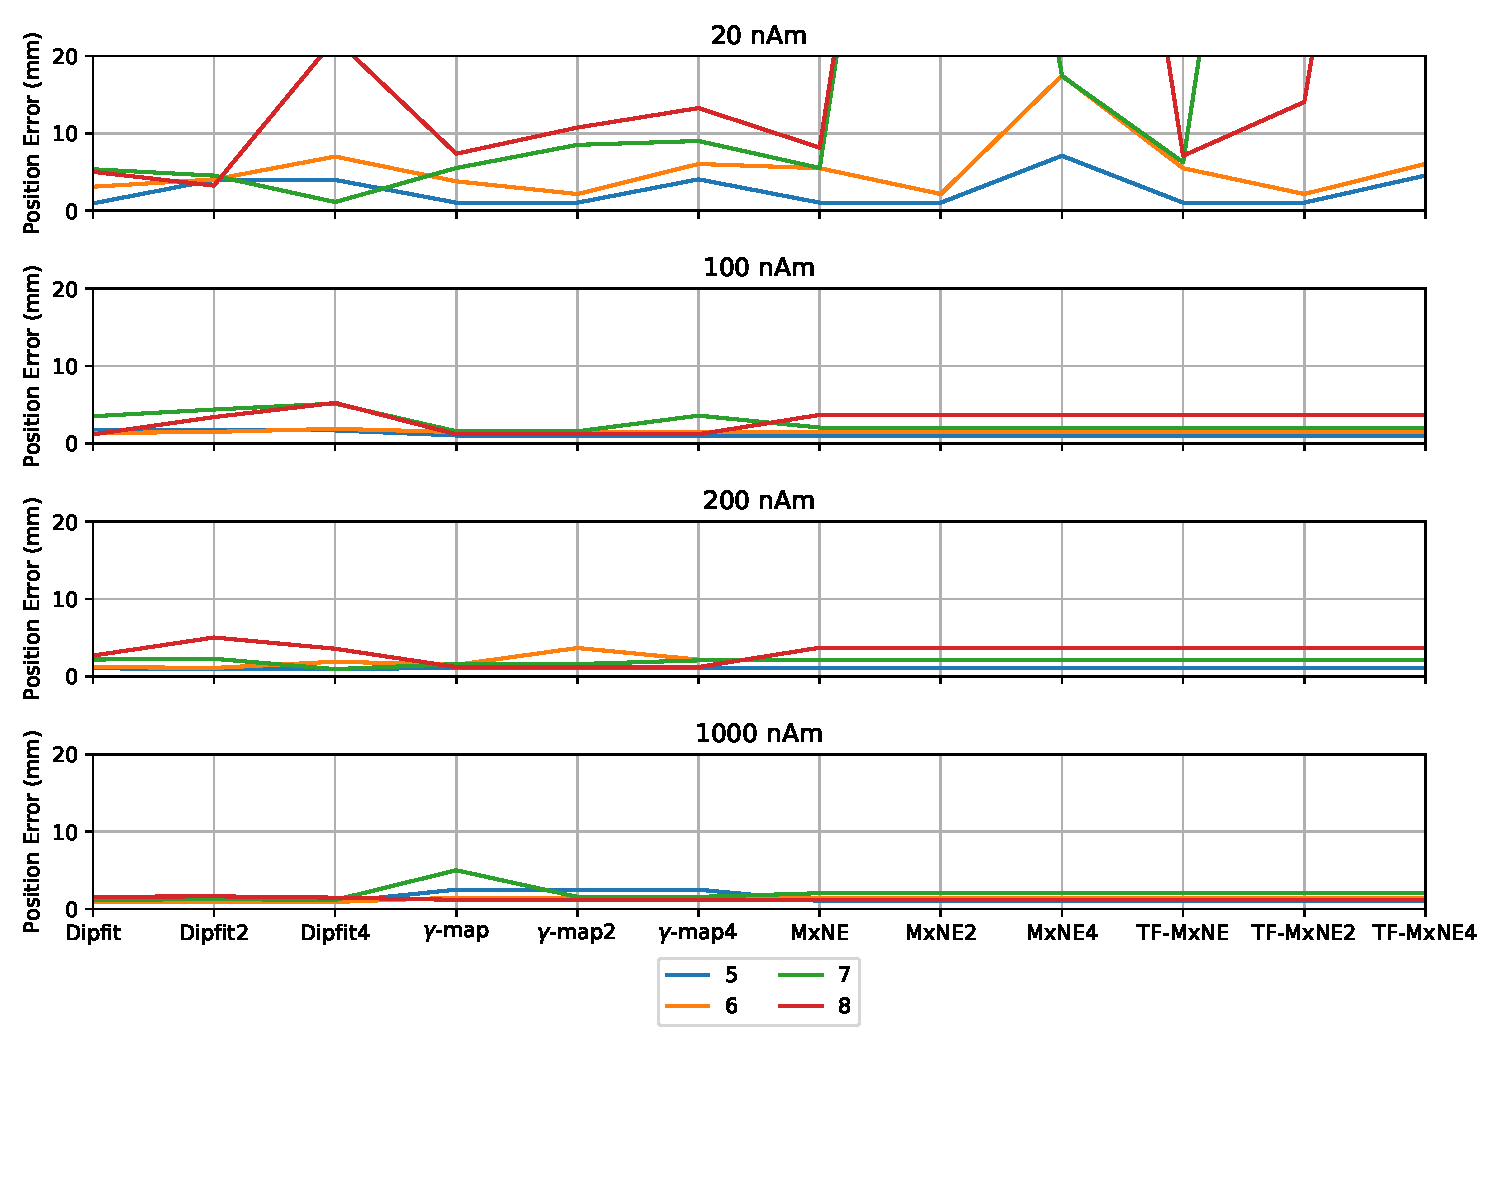
\includegraphics[trim={1cm 2.5cm 1cm 1cm},width=\textwidth]{benchmark/phantom_errors_compare_snr_in_solvers_maxfilter_True_loc_error}
            \caption{\label{fig:all_solvers_loc_error_decim}}
        \end{subfigure}
		\hspace{25pt}
        \begin{subfigure}[b]{0.47\textwidth}  
            \centering 
            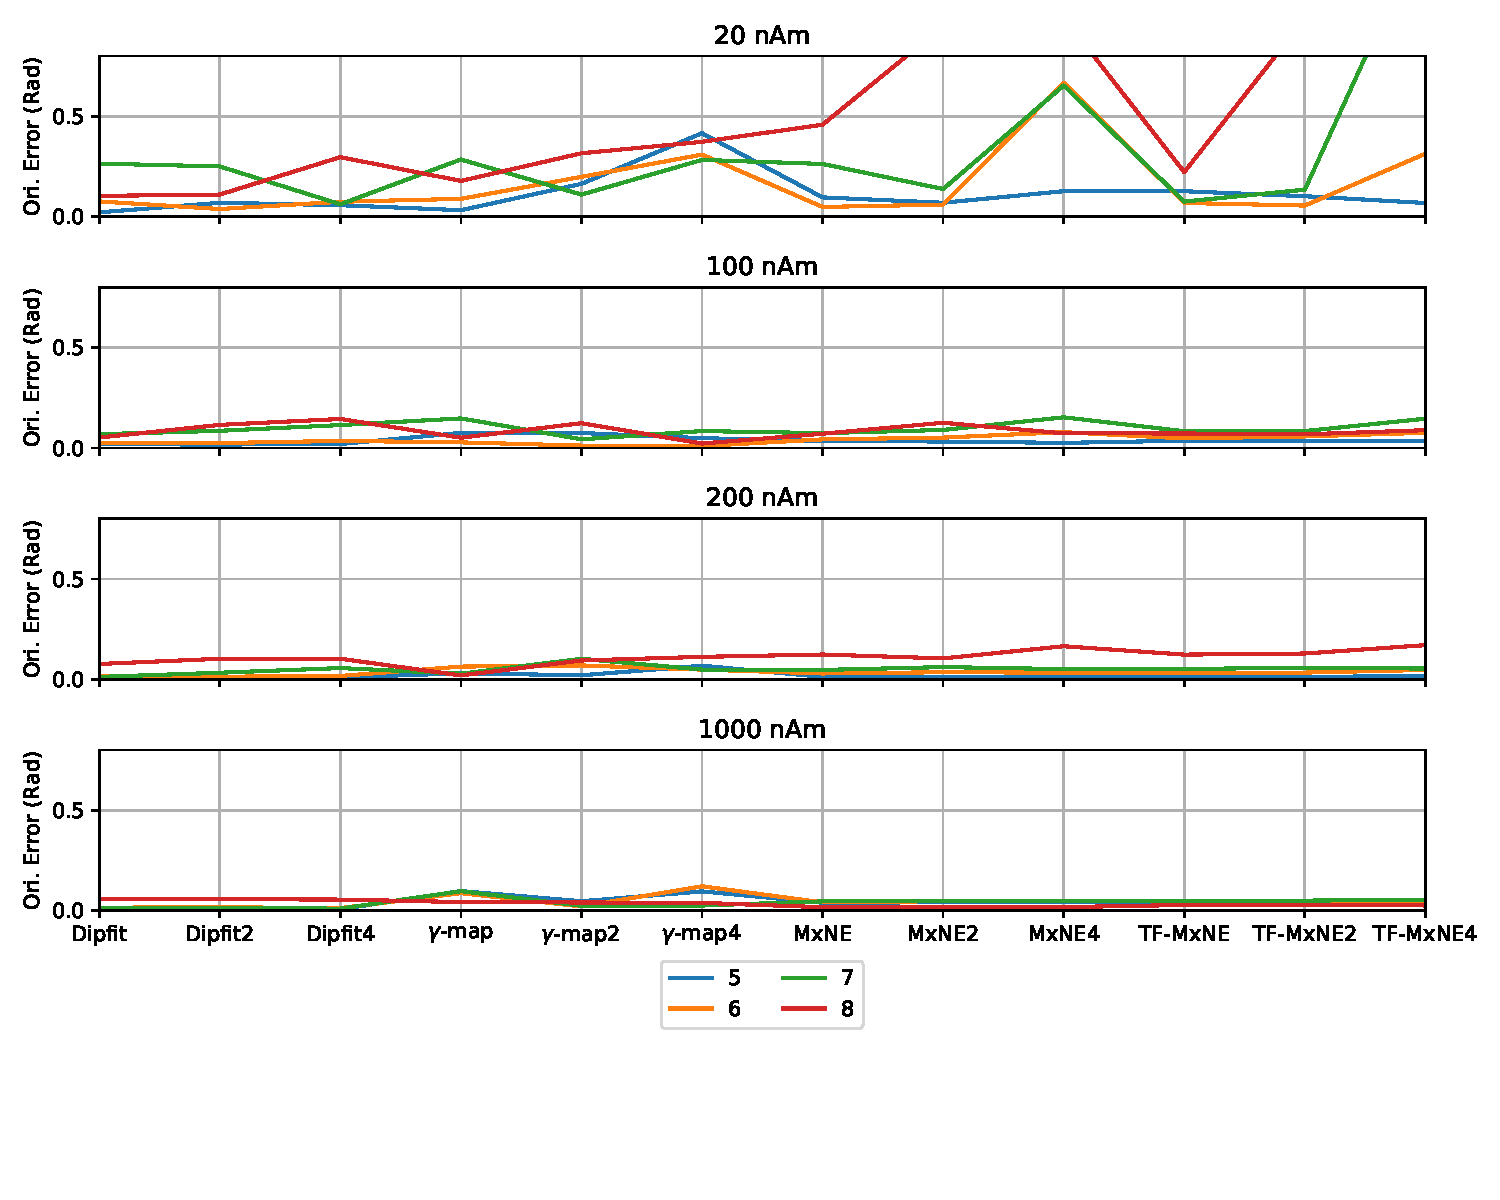
\includegraphics[trim={1cm 2.5cm 1cm 1cm},width=\textwidth]{benchmark/phantom_errors_compare_snr_in_solvers_maxfilter_True_ori_error}
            \caption{\label{fig:all_solvers_ori_error_decim}}
        \end{subfigure}

		\caption{Comparison of the position and the orientation error between come solvers when taking only part of the epochs to reduce the SNR..\label{all_solvers_loc_error_decim}}
\end{sidewaysfigure}

To investigate further the impact of each solver and the impact of a dataset with a high or a low SNR, we show in Figure~\ref{all_solvers_loc_error_decim} the results for some solvers when using all the epochs, or when decimating them into one over two epochs, or one over four epochs. Figure~\ref{fig:all_solvers_loc_error_decim} shows a deterioration of dipole fitting when using the 20nAm, especially for the case where we keep only one epoch over four. For 100nAm, 200nAm, and 1000nAm, the difference is small as the data corresponds already to a pretty strong unrealistic signal. TF-MxNE still performs better than MxNE due to the kind of simulation done in the phantom, which is basically a sinusoidal waveform, easier to be captured by the TF-MxNE.

This analysis has been performed also on two other datasets, where same kind of results can be seen in Figures~\ref{}. 

\section{Conclusion \& Perspectives}
In this chapter, the main motivation was to present some results on various source localization techniques applied to phantom data. Being able to examine "real" datasets with ground-truth is a big privilege to test the big list of existing methods for solving the MEG/EEG inverse problem.

Here we presented some of them, focusing on the approaches defined in this thesis. The conclusion would be that the dipole fitting is the most competitive and unbeatable method when having a focal dataset with only one dipole. Unfortunately here, we could not present phantom dataset with two or more dipoles in the same recording, which would make the source localization more challenging.

A further work would be to investigate this aspect of multiple dipoles. The idea would be to confirm a better performance of convex and non-convex solvers (Variational or Bayesian formulation) compared to dipole fitting or MUSIC.

This chapter also did not show any hyperparameter tuning, or an automatic estimation as shown in Chapter~\ref{chapter:bayesian}, due to the "easiness" of the dataset when having only one dipole simulated. Thus, the analysis here was always taking the best dipole estimated among the several ones picked by the solver as involved in the MEG data. This cannot be done if we had two simulated dipoles, and one would have needed to investigate clearly and properly the hyperparameter setting. In this chapter, the hyperparameters to be selected were not having a big impact on the resulted source estimate, except for the TF-MxNE where several ones needed to be fixed. The size of the window size and the time shift of the dictionary were chosen as the best ones from a grid search.